% RECOMMENDED %%%%%%%%%%%%%%%%%%%%%%%%%%%%%%%%%%%%%%%%%%%%%%%%%%%
\documentclass[graybox]{svmult}
\usepackage[hyperfootnotes=false]{hyperref}
\hypersetup{bookmarksdepth=3}
% choose options for [] as required from the list
% in the Reference Guide

\usepackage{mathptmx}       % selects Times Roman as basic font
\usepackage{helvet}         % selects Helvetica as sans-serif font
\usepackage{courier}        % selects Courier as typewriter font
\usepackage{type1cm}        % activate if the above 3 fonts are
                            % not available on your system
%
\usepackage{makeidx}         % allows index generation
\usepackage{graphicx}        % standard LaTeX graphics tool
                             % when including figure files
\usepackage{multicol}        % used for the two-column index
\usepackage[bottom]{footmisc}% places footnotes at page bottom
\graphicspath{{figures/}}
%\documentclass{article}
% \usepackage{tikz}
 \usepackage{adjustbox}
 \usepackage{multirow}
 \usepackage{algorithm}
 \usepackage{algpseudocode}
 \usepackage{ifthen}
 \usepackage{csquotes}
 \usepackage{amsmath}

\usepackage{comment}
 \usepackage{natbib}
 \setcitestyle{numbers,square}
% \usepackage{hyperref}
 \usepackage[subrefformat=parens,labelformat=simple,caption=false,labelfont={bf}]{subfig}
%\usepackage{floatrow}
 \usepackage[nolist,smaller]{acronym}
% \usepackage{nomencl}
\allowdisplaybreaks
\makeindex

\begin{document}
\begin{acronym}[ALSPAC]
  \acro{FAS}{Foetal Alcohol Syndrome}
  \acro{CPT}{Cumulative Prospect Theory}
  \acro{PT}{Prospect Theory}
  \acro{NICE}{the National Institute for Health and Care Excellence}
  \acro{IAPT}{Improving Access to Psychological Therapies}
  \acro{CMACE}{Centre for Maternal and Child Enquiries}
  \acroindefinite{CMACE}{the}{the}
  \acro{AUDIT}{Alcohol Use Disorders Identification Test}
  \acro{T-ACE}{Tolerance, Annoyance, Cut down, Eye-opener}
  \acro{RCOG}{Royal College of Obstetricians and Gynaecologists}
  \acroindefinite{RCOG}{the}{the}
  \acro{AML}{acute myeloid leukaemia}
  \acro{ADHD}{Attention Deficit Hyperactivity Disorder}
  \acro{PND}{Postnatal Depression}
  \acro{RCT}{randomised control trial}
  \acro{WHO}{the World Health Organisation}
  \acro{ESS}{Evolutionarily Stable Strategy}
  \acrodefplural{ESS}[ESS]{Evolutionarily Stable Strategies}
  \acro{MCMC}{Markov chain monte carlo methods}
  \acro{DU}{Discounted Utility}
  \acro{AIC}{Akaike information criterion}
  \acro{ANOVA}{analysis of variance}
  \acro{ALSPAC}{the Avon Longitudinal Study of Parents and Children}
  \acro{GEM}{Gaussian Emulation Machine}
  \acrodefplural{GEM}{Gaussian Emulation Machines}
  \acro{GEM-SA}{Gaussian Emulation Machine for Sensitivity Analysis}
  \acro{JIT}{Just-in-time}
  \acro{ABM}{Agent Based Modelling}
  \acro{ABMs}{Agent Based Models}
  \acro{CPT}{Cumulative Prospect Theory}
  \acro{FFH}{Fast and Frugal Heuristic}
  \acro{OFC}{orbito-frontal cortex}
  \acro{BACCO}{Bayesian Analysis of Computer Code Outputs}
  \acro{IQR}{interquartile range}
\end{acronym} 

\title*{Deciding to Disclose}
\subtitle{A Decision Theoretic Agent Model of Pregnancy and Alcohol Misuse}

\author{Jonathan Gray, Jakub Bijak, and Seth Bullock}
% Use \authorrunning{Short Title} for an abbreviated version of
% your contribution title if the original one is too long
\institute{Jonathan Gray \at University of Southampton, Southampton, United Kingdom \email{j.gray@soton.ac.uk}
\and Jakub Bijak \at University of Southampton, Southampton, United Kingdom \email{j.bijak@soton.ac.uk}
\and Seth Bullock \at University of Southampton, Southampton, United Kingdom \email{sgb@ecs.soton.ac.uk}}

\maketitle

%*************************
% Acronyms
%*************************
%\phantomsection
%\refstepcounter{dummy}
%\pdfbookmark[1]{Acronyms}{acronyms}
%\markboth{\spacedlowsmallcaps{Acronyms}}{\spacedlowsmallcaps{Acronyms}}
%\section*{Acronyms}
             
%\refstepcounter{dummy}
%\pdfbookmark[1]{Glossary}{glossary}
%\printglossary[type=main]

%\printnomenclature{}

%!TEX root = disclosure_game.tex
\begingroup
\let\clearpage\relax
\let\cleardoublepage\relax


\section*{Abstract}

We draw together methodologies from game theory, agent based modelling, decision theory, and uncertainty analysis to explore the process of decision making in the context of pregnant women disclosing their drinking behaviour to their midwives.

We employ a game theoretic framework to define a signalling game. The game represents a scenario where pregnant women decide the extent to which they disclose their drinking behaviours to their midwives, and midwives employ the information provided to decide whether to refer their patients for costly specialist treatment. This game is then recast as two games played against \enquote{nature}, to permit the use of a decision theoretic approach where both classes of agent use simple rules to decide their moves.
Four decision rules are explored - a lexicographic heuristic which considers only the link between moves and payoffs, a Bayesian risk minimisation agent that uses the same information, a more complex Bayesian risk minimiser with full access to the structure of the decision problem, and a \ac{CPT} rule.

In simulation, we recreate two key qualitative trends described in the midwifery literature for all the decision models, and investigate the impact of introducing a simple form of information sharing within agent groups.
Finally a global sensitivity analysis using \acp{GEM} is conducted, to compare the response surfaces of the different decision rules in the game.
\acresetall

\section{Introduction}
\label{sec:intro}
%CONTRIBUTION, FUCKER!
%Also, remember to say what you're going to do for the rest of the article? %(half page)

%%!TEX root = disclosure_game.tex
%Rewrite all of this, ditch the alcohol stuff altogether. Any really key can be woven in elsewhere (discussion)
\section{Previous Research}

\label{sec:lit_review}

This section presents a brief overview of previous research, addressing in turn signalling games, normative decision theory, heuristic decision making, and descriptive decision theory.


\subsection{Signalling Games}

The preponderance of classical game theory focuses on strategic decision making, in scenarios where all players have complete information about all aspects of the game. An alternative, perhaps more common situation, is that players have incomplete information, i.e. their knowledge of the rules of play is in some way deficient. \citet{Harsanyi1967} introduced the concept of a Bayesian game, resolving the problems introduced by the incomplete information scenario by allowing the possible variations on the rules to be treated as subgames. This adds an additional player - nature, to the game, where nature takes the first move thereby deciding which subgame is played. Nature is assumed to make their move by lottery, and where the probability distribution governing the lottery is known to all players this permits the game to be formulated as one of complete information. Here, we are specifically interested in signalling games \citep{Kreps1987,Spence1973}, where one player holds some private information which may be communicated (or not) by means of a signal.

This basic form has been widely applied, with substantial interest in what conditions permit honest signalling as Nash equilibria or \ac{ESS}. \citet{Grafen1990}, following from a suggestion by \citet{Zahavi1975}, proposed that if signals intended to indicate mate quality exacted a cost on the signaller (e.g. peacock tail feathers), then honest signalling would constitute an \ac{ESS}. Similar results have also been demonstrated in a game of job market signalling, where signal cost was differentiated by type \citep{Spence1973}. 
Costly signalling has also been suggested as an explaination of behaviour that at first gasp appears counter intuitive, for example \citet{Godfray1991} applied the idea to the food solicitation behaviour of chicks, where a stronger signal carries a risk of being eaten. Moving beyond animal behaviour, \citet{Sosis2003} considered the implications if ritual behaviour, in the context of religion, represented a costly signal, an idea subsequently extended by \citet{Henrich2009} to include cultural transmission, and \citet{Wildman2011} to introduce group differentiation.

Other work augments the signalling game model, for example \citet{Austen-Smith2005} adds a second `peer group' audience signalling game to the original \citeauthor{Spence1973} game in an effort to explain poor academic performance in some social groups, with some subseqent empirical support for the idea from \citet{Jr2010}. On a similar tack, \citet{Feltovich2002} introduced additional noisy type information, finding that this effectively explained counterintuitive observed behaviour where actors with every right to boast of their quality faail to do so.

\subsection{Normative Decision Theory}

Where game theory addresses strategic decision making, decision theory deals instead with rational decision making \citep{Peterson2009}.  Taken literally, this leads to normative decision theory, where the focus is on giving the rational answer to a decision problem. An alternative view - descriptive, or behavioural decisin theory, holds that the focus should instead be on giving an account of human decision making, complete with observed deviations from perfect rationality, which we address in section \ref{sub:descriptive_theories}. Finally a third perspective, which to some extent overlaps this division, suggests that decisions are heuristic in nature and rational in ecological context (section \ref{sub:heuristic_theories}).

The conceptual underpinning of all of these is the central idea of expected utility, originated by \citet{Bernoulli1954} and later formalised by \citet{Neumann1953}, which treats all decisions as gambles defined in terms of payoffs and probabilities.

Recently, several studies have explored biological correlates to aspects of expected utility. The fundamental concept, that all outcomes are comparable in a universal currency has been supported by evidence of neural correlates of decision variables \citep{Platt1999}, and following from this results from \citet{Padoa-Schioppa2006,Padoa-Schioppa2008} showing neuronal firing in the \ac{OFC} corresponding to revealed preferences in monkeys. Additionally, some support for neural representation of value, and risk aversion was found by \citet{Christopoulos2009}. The model presented in this paper makes an explicit assumption that social decisions utilise the same process, and while this is less well supported there is some evidence to suggest involvement by the same brain region, since damage to the \ac{OFC} has been shown to impair social judgements in both primates \citep{Watson2012}, and humans \citep{Willis2010}.

An alternative normative model of decision making is Bayesian decision theory, proposed by \citet{Robbins1964}, which is essentially the application of Bayesian style probabilities to the expected utility model. This allows probabilities used in reasoning to be subjective, which may allow for a better account of decisions from experience (see \citet{Hau2008,Hertwig2004} for results elucidating the distinction, and comparing the performance of several non-Bayesian models). This model has seen notable successes in practical problems \citep{McNamara1980,Survey2003,Kristensen1997}, but suggestions by several authors  that it could constitute an effective (top-down) model of learning \citep{Tenenbaum2006,Griffiths2010}, or induction \citep{Gallistel2012} in the brain have attracted substantil criticism, e.g. \citet{Bowers2012}, and \citet{Miller2012} responding to \citeauthor{Tenenbaum2006,Griffiths2010}, and \citeauthor{Gallistel2012} respectively.

\subsection{Heuristic Decision Making}\label{sub:heuristic_theories}

As noted, heuristic decision making stems from a contention that \citeauthor{Neumann1953} type rationality ignores the both context of decision making, and a lack of correspondence between predicted and actual human decisions (see, for example the Allais paradox \citep{Society2013}, and subsequent empirical support \citep{Oliver2003,Burke1996}). Arguably, this begins with \citet{Simon1956}, who suggested that humans do not attempt to make optimal choices, but to satisfice and choose the first `good enough' option. While noting that this will often achieve the same result, the claim is that humans exhibit bounded rationality \citep{Simon2000} arising from inherent limits to cognition.

\citet{Gigerenzer1996} take the concept of bounded rationality further, and argue for what they term \ac{FFH}. This recasts rationality as bound to the context of the behaviour - a rational approach to choosing the right mate might well require checking every possible partner, but given finite time, memory, and so on rapidly becomes nonsensical. On this basis, they contend that the rationality of any given decision rule can only be determined in the context of the environment, which implies that heuristics are task specific. 

\subsection{Descriptive Decision Theory}\label{sub:descriptive_theories}

While heuristic theories arguably fall under the purview of the descriptive, the wider tendency is towards what are in essence patches to normative models. The most influential models in this class derive from \ac{PT} \citep{Kahneman1979}, which combines a set of heuristics based on observed decision behaviour \citep{Tversky1974}, with distortions to the perception of probability, and the value of outcomes \citep{Kahneman1984,Tversky1986} . \citet{Tversky1992} subsequently addressed issues present in their original formulation by introducing \ac{CPT}, which allows for non-binary decisions, at the expense of the heuristics. The essence then, is that high and low probabilities are treated differently, and the subjective value of a loss differs from the equivalent gain (losing your shirt is perceived as more of a loss than winning a shirt is a gain).
This last, known as the framing effect is particularly significant, see for example work by \citet{Toll2007} examining the relationship between loss and gain framings and success rates in giving up smoking, and \ac{NICE} guidance on framing of treatment options \citep{NICE2007}.

\ac{CPT} has been successful in explaining a number of anomalous results in decision tasks (see \citet{Camerer2004a} for a review), and \citet{Thaler2000} comments to the effect that the theory is promising, albeit incomplete, lacking for example any explanation of how frames are constructed. While an effective account of decision behaviour under risk, the theory does not attempt to resolve apparent inconsistencies that arise when outcomes are delayed, i.e. in situations of intertemporal choice. Historically, \ac{DU} \citep{Samuelson1937}, which effectively claims that the value of a thing now is exponentially greater than the promise of the same thing at some future date, has been applied to explain this. More recently, \citet{Ainslie1991} has suggested that discounting of future outcomes is hyperbolic, rather than exponential, although neither model is complete - both fail to account for results from \citet{Thaler1981} showing differing temporal discounting rates for losses and gains. \citet{Loewenstein1992} report additional failings in classic \ac{DU} models, and propose a modified form of \ac{CPT} which they suggest is able to handle both immediate, and intertemporal choice.


\begin{comment}Under this model, the expected utility of any gamble is a function
of the probability of the outcomes, their utility to the gambler,
and the gambler's risk aversion. Essentially this is an extension
of the expected value criterion, which assumes that the expected value
is based only on the probability and objective value of outcomes.
By contrast, the utility framing is a subjective measure, allowing
differing preferences between gamblers. \citet{Neumann1953} later
formalised the theory, defining rational decision as acting to maximise
expected utility, where an individual's preferences are shown to fulfil
four axioms, namely completeness, transitivity, independence, and
continuity. Completeness requires that for any two lotteries A and
B, the decision maker prefers one to the other, or is indifferent.
Transitivity requires that if A is preferred to B, and B is preferred
to C, then A is also preferred to C. Continuity states that given
a scenario as in the transitivity axiom, there is some combination
of lotteries A and C where the decision maker is indifferent between
that combined lottery and B. Finally, independence maintains that
if one were to prefer gamble A to B, that preference holds if both
are combined with lottery C.

Bayesian decision theory, as expounded by \citet{Robbins1964} applies
Bayesian inference to the process of decision making under some degree
of uncertainty, where decisions may be one-shot, or repeated.
The central idea is relatively straightforward, and assumes that the
loss or gain of some action to resolve a decision is contingent on
an unknown parameter. To solve the problem, the decision maker chooses
whichever action will minimise the risk, where the risk of an action
is $\underset{i}{\sum}\lambda(a_{j}|w_{i})P(w_{i}|x)$, i.e. the loss
incurred for taking action $a_{j}$ given that the true state of the
world is $w_{i}$, multiplied by the belief that this is the true
state of world given evidence $x$, summed across all possible worlds.
Essentially this is identical with expected value, with Bayesian style
probabilities. This allows an additional process of inference to progressively
update the distribution from which $P(w_{i}|x)$ derives, as new evidence
is obtained after each decision. 

This approach has been used in a wide variety of scenarios, for example
\citet{McNamara1980} have applied statistical decision theory as
a framework for understanding animal learning%
\footnote{Although they note that this is in the sense of how animals `should'
learn, rather than how they do learn%
}, while \citet{Harsanyi1978} has derived an ethical framework from
the principles. Less controversially, in contexts where optimality
is desirable as an outcome, \citet{Survey2003} have used Bayesian
decision methods in combination with \ac{MCMC} to solve complex waterfowl
habitat management problems, and \citet{Kristensen1997} has developed
robots which utilise Bayesian decision analysis to plan sensor operations.

As with standard expected utility, the Bayesian approach can be criticised,
in this case on the grounds of plausibility. The question of plausibility
arises from the suggestion that Bayesian inference is in some way
a model of human inductive reasoning, as argued by some branches of
cognitive science. For example, \citeauthor{Tenenbaum2006} argue
for the Bayesian approach as a top-down model of inductive reasoning
in humans \citep{Tenenbaum2006,Griffiths2010}, a general approach
criticised by \citet{Bowers2012} as unfalsifiable, overcomplicated,
and relying on an unrealistic conceptualisation of the brain as optimal.
\citet{Miller2012} also applied similar criticism to claims by \citet{Gallistel2012}
that Bayesian inference better characterises learning as opposed to
associative conditioning type models, suggesting that this relies
on an assumption of optimality which is unfounded.


\subsubsection{Descriptive Decision Theory}

Arguably the most significant criticism of theories of decision making,
is their failure to correspond to empirically observed decision making
\footnote{This critique is not unique to decision theory, and has also been
levelled at game theory (e.g. \citet{Fehr2003} on the irrational
altruism of humans playing the prisoners' dilemma).%
}. This was probably first raised by \citet{Simon1956}, who proposed that the
apparent divergence derived from a tendency to satisfice, rather than
optimise. This suggestion rests on the not unreasonable assumption
that people do not have unlimited cognitive capacity (i.e. bounded
rationality \citep{Simon2000}), and hence use heuristic means to
make decisions, namely by choosing the first `good enough' option.
\citeauthor{Simon1956} suggests that this process nevertheless leads
to the optimal solution is most cases.

Subsequent work on descriptive theories largely follows the same framework
in assuming that in reality, human decision making is a heuristic
process. \citet{Tversky1974} developed three heuristics to explain
observed systematic errors in reasoning - representativeness, availability,
and anchoring. Representativeness suggests that when asked to judge
how related one object or event is to another, they do this based
on the extent to which they resemble one another - crucially they
will ignore additional, better information when available. Availability
claims that when tasked with estimating probabilities, people will
rely on the ease with which they can call examples to mind (note that
this might be considered an example of satisficing). Finally, anchoring
proposes that when estimating, people start with some initial value
and progressively update from there, i.e. they will tend to overweight
prior evidence at the expense of new information. 

Subsequently, \citet{Kahneman1984,Tversky1986} also identified framing
effects, which imply that the decisions people make are impacted by
the fashion in which the problem is presented. The essential outcome
from these findings is that people are risk seeking when faced with
outcomes framed as losses, but risk averse towards gains, and regard
any loss as greater than an equivalent gain. The impact of framing
in itself has been shown to be significant, for example \citet{Toll2007}
found improved abstinence rates in smoking cessation where quitting
was framed as a gain, and \ac{NICE} recommend considering the framing
of treatment outcomes when presenting options to patients \citep{NICE2007}.

\ac{PT} \citep{Kahneman1979} attempts to provide a decision rule
accounting for the heuristic nature of decision making and incorporate
framing effects, which successfully explains many perceived failures
of rationality. A revised version, \ac{CPT} \citep{Tversky1992}
addressing a violation of first order stochastic dominance possible
under the original formulation, extends the theory to allow decisions
with more than two options, but sacrifices the editing phase. \citet{Camerer2004a}
reviews a number of successes in explaining apparent anomalies with
\ac{CPT}, and argues that should replace expected utility in general
usage. \citet{Thaler2000} regards the theory as promising, but points
out that it is in many ways incomplete, citing the lack of explanation
as to how people construct frames as an example of this.

A significant weakness of \ac{CPT} as a general theory of decision
making is that it fails to account for behaviour under intertemporal
choice, or rather does not attempt to address it. Generally, intertemporal
choice is assumed to be underpinned by the \ac{DU} model of \citet{Samuelson1937},
which proposes that the value of a thing right now is greater than
the value of it at some point in the future (jam today has more utility
than jam tomorrow), following an exponential relationship. A more
nuanced view of this has been proposed by \citet{Ainslie1991}, suggesting
that the relationship is hyperbolic rather than exponential. Both
models however fail to explain several inconsistencies, for example
\citet{Thaler1981} found that discounting rates were different between
gains and losses. \citet{Loewenstein1992} report a number of additional
inconsistencies that are not adequately resolved by \ac{DU} models,
and propose an alternative along the lines of \ac{CPT} to resolve
them while retaining the capabilities of Kahneman and Tversky's model
in immediate term choices.
\end{comment}
%\section{Approach and Motivation}
\label{sec:model_design}

The appropriate game representative of the scenario of interest, which captures the desired strategic dynamics may not be immediately obvious. There will almost invariably be many possible alternatives, of which some are isomorphisms, and others fundamentally different conjectures about the data generating process. I would suggest that an iterative process is beneficial, beginning from the simplest possible game, and progressively augmenting it.

Transitioning from the resulting game, to a set of decision problems is a relatively simple task. I have treated the $n$ player game as $n$ one-player games \citep{RiosInsua2009}, where the moves of other players are drawn from a probability distribution - nature, in game theoretic parlance. As with the game, the decision problem representation admits a degree of variation, and may need to be adjusted to reflect the decision rules that will be used.

These decision problems may then form the basis of an agent model, where agents use learning, and decision rules to play out the game. Simulation can then support features which are not readily representable within an analytic framework, for example, populations of heterogeneous players, individual and social learning, or network effects. In addition, the ability to observe the system in a state of flux rather than at equilibrium is desirable, since even where a social system reaches a stable state, the process by which we arrive at it is significant. 
%!TEX root = disclosure_game.tex
\section{Disclosure Game Model}
\label{sec:model}
%Start this off with a brief description of our fictional scenario.
% Whole section ~ 1.5K

In this section we outline the disclosure game model, and give details of the four decision rules, but begin with a brief sketch of a pregnancy in terms of encounters between a woman and a midwife. 

Typically women will have 12 appointments with a midwife during the antenatal period. Outside of caseloading teams, a woman does not generally have a named midwife, and may see a different practitioner at each appointment. In the UK, and unlike most healthcare scenarios, maternity notes are patient held, so midwives do not have extensive information prior to an appointment unless they have encountered the woman previously. Maternity notes are not generally linked to extra-departmental records, meaning that a history of alcohol related admissions to another service may remain unknown unless revealed by the woman.

According to NICE guidance \citep{NICE2010a,NICE2010} substance misuse should be raised at the initial booking appointment, and subsequent action if a concern is raised is at the discretion of the midwife. This may take the form of specific guidance to reduce intake, or if deemed necessary a referral to a specialist midwife and relevant interdisciplinary team. On alcohol consumption, policy regarding how to determine the level of consumption is generally at the trust level, or according to the best judgement of the individual midwife, with no guidance provided by NICE. This commonly takes the form of average units per week, but may include \ac{T-ACE} and similar measures. 

Beyond the booking appointment, the onus is on women to raise concerns about their drinking behaviour, or the midwife to probe further if they feel it is warranted. In either case, once a concern has been raised the midwife must respond clinically, and inevitably personally, to the information.

In an ideal world, all interactions with healthcare providers would be immediately and fully disclosive, with no repercussions for the patient. However, alcohol misuse by women is known to attract stigma \citep{Gomberg1988}, and is a recognised barrier to appropriate treatment in the maternity context \citep{Radcliffe2011,NICE2010}.

\subsection{Disclosure Game}
\label{sub:the_game}
%Outline how the scenario translates into a game.
%Brief mention of the game theoretic solution

In order to translate the scenario sketched above into a more abstract, tractable form, we cast it as a signalling game, and assume that women's disclosures (or not), are signals. We also make the simplifying assumption that a woman may have one of only three drinking patterns - light, moderate, or heavy. Correspondingly, they are limited in what signals they may send to claiming to be one of these three types.

Midwives are treated in a similar fashion, where their type corresponds to how negatively they regard a drinking pattern - non-judgemental, moderately judgemental, and harshly judgemental. The expression of this judgement is not a matter of choice on their part, and is assumed to have no impact on their response, which is to either refer the woman for specialist treatment, or do nothing.

At the end of a game, each player receives a payoff dependent on the actions and types of both players, which has a partially common interest component. Women receive a payoff based on the health of their eventual baby, with a social cost dependent on the signal they sent and the midwife's reaction to it. Midwives receive the same health payoff as the women, but pay a cost for referring to a specialist, mirroring the organisational cost of non-routine care. Table \ref{tab:Payoff-matrix} shows the three payoff matrices which together describe the game.

Taken together, this leads to a game tree that is relatively complex (figure \ref{fig:simple_tree} shows a simplified representation, with a detailed view of one branch in figure \ref{fig:zoom_tree}) even at the subgame level. Rather than attempt to solve for equilibria, agents treat this two player game as taking place against nature, along the lines of adversial risk analysis \citep{RiosInsua2009}. This effectively translates the game to a pair of decision problems (figure \ref{fig:decision_problems}), which agents attempt to resolve at each turn using a simple decision rule, given their prior beliefs and experience of play.

\begin{figure}[H]
\begin{adjustbox}{center}
\includegraphics[width=0.43\paperwidth]{figures/rounded_clover_infosets}
\end{adjustbox}
\caption{Simplified game tree.}

\label{fig:simple_tree}
\end{figure}

\begin{figure}[H]
\begin{adjustbox}{center}
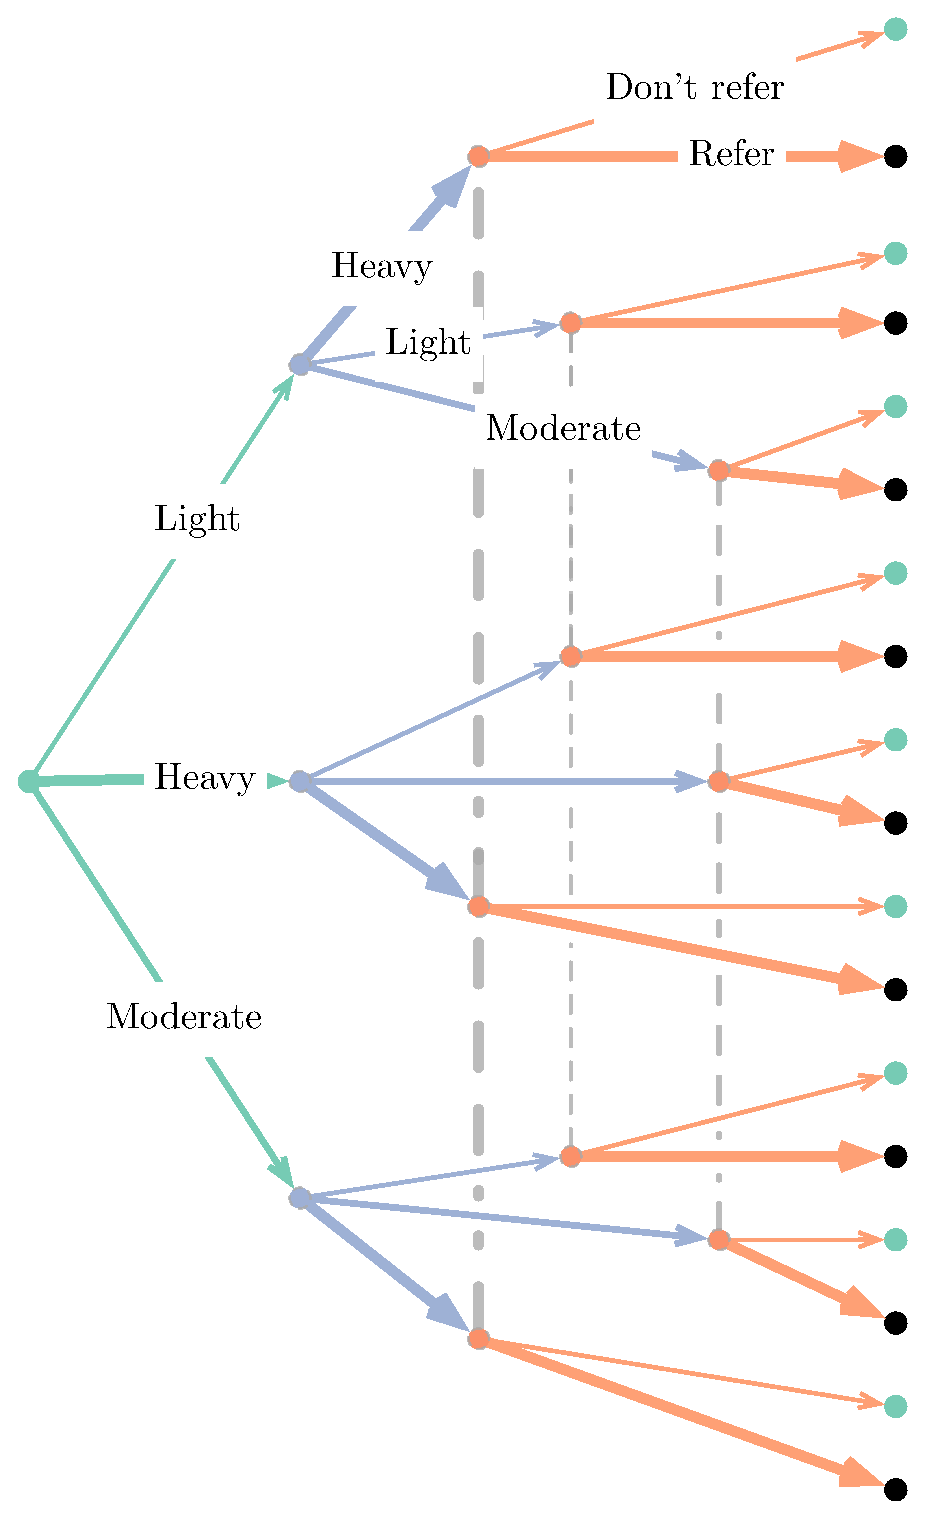
\includegraphics[width=0.43\paperwidth]{figures/tree_zoom}
\end{adjustbox}
\caption{Detail view of a single game tree branch.}

\label{fig:zoom_tree}
\end{figure}

\begin{figure}[H]
\begin{adjustbox}{center}\subfloat[Women]{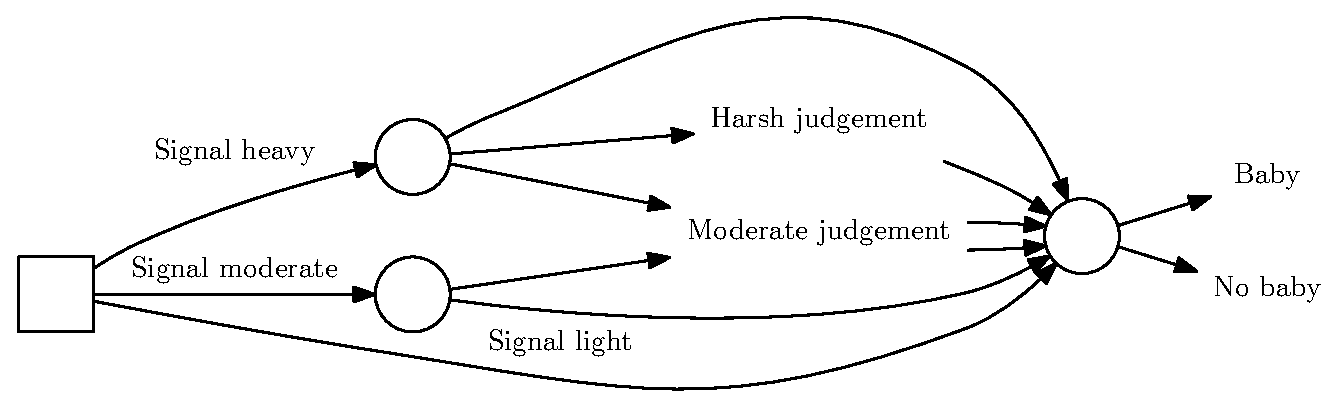
\includegraphics[width=0.43\paperwidth]{figures/women_influence}

}\subfloat[Midwives]{\includegraphics[width=0.43\paperwidth]{figures/mw_influence}}\end{adjustbox}
\caption{Influence diagrams, showing the game broken into two decision problems.}

\label{fig:decision_problems}
\end{figure}

%Might belong in a more methody bit? Read some stuff to check..
Women are drawn in order from a queue, and play against a midwife chosen at random. They play for a maximum of \(r_{w}\) rounds (\(r_{w}=12\) following the routine number of ante-natal appointments in the UK \citep{NICE2010a}) or until they are referred. At which point a new player is drawn from the same distribution that produced the original players to replace them. If they are not referred, they rejoin the back of the queue after their appointment. In either case, they are informed of their payoff after each round and update their beliefs accordingly.

Midwives play for \(r_{m}\) rounds (\(r_{m}=1000\) in all experiments), and conduct appointments in parallel, i.e. if there are 5 midwives, then five women are drawn from the queue and assigned at random to the midwives. 
Unlike women, midwives are only informed of their payoff if they choose to make a referral. Both groups of agents have perfect recall, and midwives are assumed to retrospectively update their observations if they make a referral after a number of appointments.


Formally then, let \(N = \{m, w\}\) be the set of players each with a private type \(\theta_{i} \in \Theta\), and a set of types \(\Theta=\{l, m, h\}\), with pure strategies \(A_{m}=\{r,n\}, A_{w}=\{l, m, h\}\). Additionally define a utility function \(u_{i}(s_{w}, s_{m}, \theta_{w}, \theta_{m})=X_{s, s_{w}, \theta_{m}} + X_{h, \theta_{w}, s_{m}} + X_{c, \theta_{w}, s_{m}}\), and distributions over types \(p_{w}(l, m, h)\), \(p_{m}(l, m, h)\).

\begin{table}
\center
\subfloat[Social cost, \(X_{s}\)\label{tab:Social-cost-matrix}]{%
\begin{tabular}{|c|c|c|c|c|}
\cline{3-5} 
\multicolumn{2}{c}{} & \multicolumn{3}{|c|}{Woman}\tabularnewline

\hline
\multirow{4}{*}{\rotatebox[origin=c]{90}{Midwife}} &  & Heavy & Moderate & Light\tabularnewline
\cline{2-5} 
 & Harsh & 0, -2 & 0, -1 & 0, 0\tabularnewline
\cline{2-5} 
 & Medium & 0, -1 & 0, 0 & 0, 0\tabularnewline
\cline{2-5} 
 & Low & 0, 0 & 0, 0 & 0, 0\tabularnewline
\hline 
\end{tabular}

}

\subfloat[Health outcome, \(X_{h}\)\label{tab:Referral-payoff-matrix}]{%
\begin{tabular}{|c|c|c|c|c|}
\cline{3-5} 
\multicolumn{2}{c}{} & \multicolumn{3}{|c|}{Woman}\tabularnewline

\hline 
\multirow{3}{*}{\rotatebox[origin=c]{90}{Midwife}} &  & Heavy & Moderate & Light\tabularnewline
\cline{2-5} 
 & Refer & 10, 10 & 10, 10 & 10, 10\tabularnewline
\cline{2-5} 
 & Don't refer & -2, -2 & -1, -1 & 10, 10\tabularnewline
\hline 
\end{tabular}

}

\subfloat[Referral cost, \(X_{c}\)\label{tab:inst_cost_matrix}]{%
\begin{tabular}{|c|c|c|c|c|}
\cline{3-5}  
\multicolumn{2}{c}{} & \multicolumn{3}{|c|}{Woman}\tabularnewline
\hline 
\multirow{3}{*}{\rotatebox[origin=c]{90}{Midwife}} &  & Heavy & Moderate & Light\tabularnewline
\cline{2-5} 
 & Refer & -9, 0 & -9, 0 & -9, 0\tabularnewline
\cline{2-5} 
 & Don't refer & 0, 0 & 0, 0 & 0, 0\tabularnewline
\hline 
\end{tabular}

}

\caption{Payoff matrices\label{tab:Payoff-matrix}}
\end{table}

\subsection{Agent Models}
\label{sub:the_agents}
%Outline basic structure, then specifics on each one.
%This should probably go lexic -> bayes payoff -> bayes -> CPT in order
% of complexity.
%suggest there are added shells of complexity
%		mention the info sharing because homophilly
%			related - the enhancement to the bayes/cpt agents is that they personalise, as much as anything.
%		properly explain dirichlet priors
% How about comparing the decision problem representation for the agent types?

While in principle a wide variety of agent models are possible, given that decision rules operate on essentially the same information, and produce the same outputs, we limit ourselves here to four. The simplest is a lexicographic rule (1), motivated as in the spirit of a \ac{FFH} \citep{Gigerenzer2004} which uses only information about payoffs given actions; a Bayesian risk minimisation rule using the same information (2); a second Bayesian risk rule (3) which uses information about the underlying lottery; and a two-stage \ac{CPT} \citep{Hau2008} agent (4) which is identical with 3, but uses the \ac{CPT} decision rule from \cite{Tversky1992}. Hence, each successive decision model adds a layer of sophistication to the problem representation while retaining the same input-ouput characteristics.

As noted in section \ref{sub:the_game}, agents have perfect recall, and midwives recognise women if they encounter them subsequently. While agents recall perfectly and make use of the new information for retrospective updates, all four agent models make decisions `as-if' they were always facing a new opponent.

A simplifying assumption is made that all midwives have just qualified after receiving identical training. As a result, they have homogenous beliefs about their women and assume to some extent that they are honest.
Women are heterogenous in their prior observations, which are assigned stochastically and constrained such that they have encountered each scenario possible at least once, with exactly \(k\) encounters overall.


\subsubsection{Lexicographic Heuristic}
\label{sub:lexico}

The lexicographic heuristic (algorithm \ref{alg:lexico}) follows the form of that used in \cite{Hau2008}, and assumes a simplified, where an action is a choice between combined lotteries. Functionally, the heuristic maintains a count of the number of times that each action was followed by a payoff, and chooses the action which most commonly has the best payoff, i.e. one reason decision making. This approach requires minimal computation, and does not assume that \(u_{i}\) is static, or known.

Women resolve this by approximating the utility function, as a function \(f(s_{w}, \sigma)\) on their choice of signal and an unknown distribution, which maps to \(u_{w}\) - i.e. \(s_{w}\) is a choice between simple lotteries. The algorithm maintains a count, \(n\), of the number of occurrences of each outcome given the choice from \(s_{w}\).

Midwives solve a slightly different problem with more information, where \(s_{w}\) is known, and \(s_{m}\) is the lottery choice - \(f(s_{w}, s_{m},\sigma)\). This is resolved by maintaining a separate count for each signal (i.e. \(n_{s_{w},s_{m}}\)), and otherwise following the same algorithm.

\begin{algorithm}
\begin{algorithmic}
\State n=1, action=none
\While{action is none}
\State Calculate the nth most common outcome following each action.
\State Sort actions by the value of the nth most common outcome.
\If{clear winner} \State action = best \EndIf
\State n = n + 1
\EndWhile
\State \Return action
\end{algorithmic}
\caption{Lexicographic heuristic\label{alg:lexico}}
\end{algorithm}

\subsubsection{Bayesian Payoff}

The Bayesian payoff agent uses the same subset of information as the lexicographic method, but updates beliefs on the link between actions and payoffs using Bayes rule, and attempts to choose the action which minimises risk.

Given the discrete nature of actions and payoffs, coupled with a desire for tractability of the
simulation, the Dirichlet distribution is employed to represent these beliefs. The probability
density function takes the form -

\[
D(\Theta|\alpha)=\frac{\Gamma(\sum_{i=1}^{k}\alpha_{i})}{\prod_{i=1}^{k}\Gamma(\alpha_{i})}\overset{k}{\underset{i=1}{\prod}\Theta_{i}^{\alpha_{i-1}}}
\]


Where \(\alpha=\{\alpha_{1}\ldots\alpha_{k}\}\), \(k\) is the number
of signal-payoff pairs, \(\Theta=\{x_{1},\,\ldots,x_{k-\text{1}}\}\) all
more than zero and summing to less than 1, and \(\alpha_{i}\) is the 
psuedo-count of prior observations for a pair \(i\). 

The distribution is particularly convenient, in that to infer the
probability of a signal implying a payoff becomes
simply -

\begin{equation}
P(x=j|D,\alpha)=\frac{\alpha_{j}+n_{j}}{\sum_{j}(\alpha_{j}+n_{j})}\label{eq:posterior}
\end{equation}


Where \(n_{j}\) is simply the count of occurrences of pair \(j\), so
that the belief that a signal \(j\) the number
of times that type has been observed (including the pseudo-count),
over the total number of observations thus far. This makes computation
of beliefs fast and simple, since all that must be maintained is
a count of observations with no particular concern as to their order.
As before, midwives follow a similar pattern but per signal.

Agents then choose $s_{i}$ to minimise $R_{i}$, which is simply - 
\begin{equation}
R_{w}(s_{w}) = \sum_{x \in X} -xp(x | s_{w})
\end{equation}
\begin{equation}
R_{m}(s_{w}, s_{m}) = \sum_{x \in X} -xp(x | s_{w}\wedge s_{m})
\end{equation}

Where $X$ is the set of payoffs the agent has observed to follow $s$.

\subsubsection{Bayesian Risk Minimisation}

The second Bayesian agent augments the reasoning of the simple payoff model, making the stronger assumption that the utility function is static, and known. Women maintain two sets of beliefs, corresponding respectively to \(p_{m}\), and the probability of referral given signal choice. This leads to the risk function -

\begin{equation}
R_{w}(s_{w}, \theta_{w}) = \sum_{i\in A_{m}}\sum_{j\in \Theta} -u_{w}(s_{w}, i, \theta_{w}, j)p(j)p(i | s_{w})
\end{equation}

So that the risk of a signal is the sum of the products of all payoffs with the probabilities of their entailed midwife types and responses.

Midwives reasoning centers on determining the meaning of signals, since given the knowledge of what some signal \(i\) conveys about the true type of the sender, the payoff for an action is known. As such, their inference process is the same as for the simple Bayesian agent but over signal-type pairs, and they attempt to minimise -

\begin{equation}
R_{m}(s_{w}, s_{m}) = \sum_{i\in \Theta} -u_{w}(s_{w}, s_{m}, i, \theta_{m})p(i | s_{w})
\end{equation}

\subsubsection{Descriptive Decision Theory}

The most complex decision rule used is \ac{CPT}, which attempts to reproduce a number of systematic deviations from rationality observed in humans. While \ac{CPT} has primarily been applied in the context of decisions from description, it has been modified to deal with decisions from experience by incorporating a first stage where probabilities are estimates from observations as in \cite{FoxCPT}. In this instance the Bayesian inference process fills the first stage role.

%Maybe cut this bit and make explanation richer?
Rather than the psychologically more interesting \ac{PT}, the \ac{CPT}
decision rule is used in this instance, because of the requirement
for women to evaluate more than two `prospects'.\footnote{Where a prospect is a payoff-probability pair, with the set of prospects for an action defining the possible outcomes for it.} \ac{CPT} uses transformed probabilities, underweighting
small probabilities, and overweighting large ones. This is intended to reflect the observed behaviour of humans, where sufficiently high likelihoods are treated as certain, and contrastingly low probabilities as impossible. The correct weighting function is subject to some debate, but here we have used that of \citet{Tversky1992}, which treats probabilities differently for gains and losses -

\begin{eqnarray*}
w^{+}(p) & = & \frac{p^{\gamma}}{(p^{\gamma}+(1-p)^{\gamma})^{\frac{1}{\gamma}}}\\
w^{-}(p) & = & \frac{p^{\delta}}{(p^{\delta}+(1-p)^{\delta})^{\frac{1}{\delta}}}
\end{eqnarray*}


Where $p$ is the unweighted probability, and $\gamma$ and $\delta$
are the weights for gain and loss probabilities respectively. Along similar lines, the values of losses and gains are transformed to reflect a tendency to regard a loss as more significant than a gain  -

\[
v(x)=\begin{cases}
f(x) & if\, x>0\\
0 & if\, x=0\\
g(x) & if\, x<0
\end{cases}
\]


Where,

\[
f(x)=\begin{cases}
x^{\alpha} & if\,\alpha>0\\
ln(x) & if\,\alpha=0\\
1-(1+x)^{\alpha} & if\,\alpha<0
\end{cases}
\]
\[
g(x)=\begin{cases}
-(-x)^{\beta} & if\,\beta>0\\
-ln(-x) & if\,\beta=0\\
(1-x)^{\beta}-1 & if\,\beta<0
\end{cases}
\]


And $\alpha$, and $\beta$ are respectively the power of a gain,
and a loss, and \(x=u_{i}\). The \ac{CPT} value of outcome $x$ is $v(x)w^{+}(x)$
if $x\geq0$, and $v(x)w^{-}(x)$ otherwise. For an action the \ac{CPT}
value is the sum of the value of the prospects of that action, as
in the Bayesian risk model, and the agent chooses the option which maximises this quantity.

\subsection{Information Sharing}
\label{sub:info_sharing}

It would seem unreasonable to suppose that neither party recounts their experiences to their peers, and to explore the impact of this we also modify the game to introduce a simple form of information sharing within agent groups. This takes the form of having each agent share their memories with their colleagues with some probability \(q\). Individuals then incorporate shared information into their beliefs using weighted updates, such that a shared observation of a low type signal contributes to their beliefs by \(w\), and \(0\leq w\leq 1\) (i.e. \(n_{j} = n_{j} + w\)).
Women share only when they have finished play, and provide their complete history of games, because they have accurate information about the outcomes. By the same rationale, midwives share only their history with the most recent woman they referred. Sharing occurs simultaneously for all players at the end of each round, and all memories are either shared immediately or discarded.\footnote{Memories of games remain, but it is assumed that only current news is relevant.}

Because of their differing problem representations, the simple payoff reasoners and their more complex counterparts incorporate this exogenous information differently. The simple payoff based rule relys on a belief structure relating actions directly to rewards. Because payoffs differ by the agent's private type, the information shared may not correspond to the experience of the listening agent in the same scenario. As a result, payoff reasoners have a belief bias towards the most common player type, and can believe in outcomes that are, for them, impossible.

By contrast, representing the problem in terms of the probabilities of the individual lotteries yields a structure that abstracts the new information from payoffs, and allows the agent discount implausible outcomes. This stronger assumption as to the static and known qualities of payoffs does however reduce the flexibility of the decision rule.
\subsection{Agent Models}
\label{sub:the_agents}
%Outline basic structure, then specifics on each one.
%This should probably go lexic -> bayes payoff -> bayes -> CPT in order
% of complexity.
%suggest there are added shells of complexity
%		mention the info sharing because homophilly
%			related - the enhancement to the bayes/cpt agents is that they personalise, as much as anything.
%		properly explain dirichlet priors
% How about comparing the decision problem representation for the agent types?

While in principle a wide variety of agent models are possible, given that decision rules operate on essentially the same information, and produce the same outputs, we limit ourselves here to four. The simplest is a lexicographic rule (1), in the spirit of a \acl{FFH} \citep{Gigerenzer2004} which uses only information about payoffs given actions; this is followed by a Bayesian risk minimisation rule (2) using the same information; a second Bayesian risk rule (3) which uses information about the underlying lottery; and a two-stage \ac{CPT} \citep{Hau2008} agent (4) which is identical to 3, but uses the \ac{CPT} decision rule from \cite{Tversky1992}. Hence, each successive decision model adds a layer of sophistication to the problem representation while retaining the same input-output characteristics.

Agents have perfect recall, midwives recognise women if they repeatedly encounter them, making use of new information for retrospective updates. However, all four agent models make decisions `as-if' they were always facing a new \enquote{opponent}.

A simplifying assumption is made that all midwives have just qualified after receiving identical training. As a result, they have homogeneous beliefs about  women and assume to some extent that they are honest.
Women have heterogeneous beliefs, which correspond to experiencing \(k\) randomly chosen paths through the game, and following each path at least once.


\subsubsection{Lexicographic Heuristic}
\label{sub:lexico}

The lexicographic heuristic (algorithm \ref{alg:lexico}) follows the form of that used in \cite{Hau2008}, and assumes a simplified problem representation, where an action is a choice between combined lotteries. Functionally, the heuristic maintains a count of the number of times that each action was followed by a payoff, and chooses the action which most commonly has the best payoff, i.e. one reason decision making. Where there is no clear best action, but one or more is evidently worse, a choice must be made as to whether to discard the poorer action; in this case we have elected to retain it.
This approach requires minimal computation, and does not assume that \(u_{i}\) is static, or known.

Women resolve this by approximating the utility function, as a function \(f(s_{w}, \sigma)\) on their choice of signal and an unknown distribution $\sigma$, which maps to \(u_{w}\) - i.e. \(s_{w}\) is a choice between simple lotteries. The algorithm maintains a count, \(n\), of the number of occurrences of each outcome given the choice from \(s_{w}\).

Midwives solve a slightly different problem with more information, where \(s_{w}\) is known, and \(s_{m}\) is the lottery choice - \(f(s_{w}, s_{m},\sigma)\). This is resolved by maintaining a separate count for each signal (i.e. \(n_{s_{w},s_{m}}\)), and otherwise following the same algorithm (\ref{alg:lexico}).

\begin{algorithm}
\begin{algorithmic}
\State $n \gets 1, action \gets none$
\While{$action = none$}
\State Calculate the $n$th most common outcome following each action.
\State Sort actions by the value of the $n$th most common outcome.
\If{clear winner} \State $action \gets best$ \EndIf
\State $n \gets n + 1$
\EndWhile
\State \Return action
\end{algorithmic}
\caption{Lexicographic heuristic\label{alg:lexico}}
\end{algorithm}

\subsubsection{Bayesian Payoff}

The Bayesian payoff agent uses the same subset of information as the lexicographic method, but updates beliefs on the link between actions and payoffs using the Bayes rule, and attempts to choose the action which minimises risk.

Given the discrete nature of actions and payoffs, coupled with a desire for tractability of the
simulation, the Dirichlet distribution is employed as a prior to represent these beliefs. 
The distribution is particularly convenient, in that to infer the
probability of a signal implying a payoff is
simply -

\begin{equation}
p(x=j|D,\alpha)=\frac{\alpha_{j}+n_{j}}{\sum_{j}(\alpha_{j}+n_{j})}\label{eq:posterior}
\end{equation}


Where \(n_{j}\) is simply the count of occurrences of signal-payoff pair \(j\), and \(\alpha_{i}\) is the pseudo-count of prior observations\footnote{Psuedo-counts are related to, but distinct from prior beliefs. Here, the psuedo-count is a parameter to the prior belief distribution and is nothing more than a hypothetical count of prior observations.} for a pair \(i\). Hence,
the belief that a signal will lead to a payoff is the number
of times that pairing has been observed (including the pseudo-count),
over the total number of observations thus far. This makes computation
of beliefs fast and simple, since all that must be maintained is
a count of observations.
As before, midwives follow a similar pattern but maintain \(n_{s_{w}}\) independent counts of pairings between referral choice and payoff, updating their beliefs about the relationship between the choice to refer and payoff given the signal they have received.

Agents then choose the strategy $s_{i}$ to minimise risk $R_{i}$, which is simply defined as - 
\begin{equation}
R_{w}(s_{w}) = \sum_{x \in X} -xp(x | s_{w})
\end{equation}
\begin{equation}
R_{m}(s_{w}, s_{m}) = \sum_{x \in X} -xp(x | s_{w}\wedge s_{m}),
\end{equation}

where $X$ is the set of payoffs the agent has observed to follow $s_{i}$.

\subsubsection{Bayesian Risk Minimisation}

The second Bayesian agent augments the reasoning of the simple payoff model, making the stronger assumption that the utility function is static, and known. Women maintain two sets of beliefs, corresponding respectively to \(p_{m}\), and the probability of referral given signal choice. This leads to the risk function, minimised with respect to \(s_{w}\) -

\begin{equation}
R_{w}(s_{w}, \theta_{w}) = \sum_{i\in A_{m}}\sum_{j\in \Theta} -u_{w}(s_{w}, i, \theta_{w}, j)p(j)p(i | s_{w}),
\end{equation}

so that the risk of a signal is the sum of the products of all payoffs with the probabilities of their entailed midwife types and responses.

Midwives reasoning centres on determining the meaning of signals, since given the knowledge of what some signal \(s_{w}\) conveys about the true type of the sender, the payoff for an action is known. As such, their inference process is the same as for the simple Bayesian agent but over signal-type pairs, and they attempt to minimise the following risk function, minimised with respect to \(s_{m}\) -

\begin{equation}
R_{m}(s_{w}, s_{m}) = \sum_{i\in \Theta} -u_{m}(s_{w}, s_{m}, i)p(i | s_{w})
\end{equation}

\subsubsection{Descriptive Decision Theory}

The most complex decision rule used is \ac{CPT}, which attempts to reproduce a number of systematic deviations from rationality observed in humans. Rather than risk, `prospects', the sequence of payoff-probability pairings in ascending order of payoff, associated with an action  are used as decision criteria. While \ac{CPT} has primarily been applied in the context of decisions from description, it has been modified to deal with decisions from experience by incorporating a first stage where probabilities are estimates from observations \cite{FoxCPT}. In this instance the Bayesian inference process fills the first stage role.

%Maybe cut this bit and make explanation richer?
\ac{CPT} uses transformed probabilities, underweighting small probabilities, and overweighting large ones. This is intended to reflect the observed behaviour of humans, where sufficiently high likelihoods are treated as certain, and contrastingly low probabilities as impossible. The correct weighting function is subject to some debate, but here we have used that of \citet{Tversky1992}, which treats probabilities differently for gains (eqn \ref{eqn:cpt_p_pos}) and losses (eqn \ref{eqn:cpt_p_neg}) -

\begin{align}
w^{+}(p) & = \frac{p^{\gamma}}{(p^{\gamma}+(1-p)^{\gamma})^{\frac{1}{\gamma}}}\label{eqn:cpt_p_pos}\\
w^{-}(p) & = \frac{p^{\delta}}{(p^{\delta}+(1-p)^{\delta})^{\frac{1}{\delta}}}\label{eqn:cpt_p_neg},
\end{align}


where $p$ is the unweighted probability, and $\gamma$ and $\delta$
are the weights for gain and loss probabilities respectively. Along similar lines, the values of losses and gains are transformed to reflect a tendency to regard a loss as more significant than a gain  -

\begin{equation}
v(u_{i})=\begin{cases}
f(u_{i}),& \text{if}\, u_{i}>0\\
0,& \text{if}\, u_{i}=0\\
\lambda g(u_{i}),& \text{if}\, x<0
\end{cases},
\end{equation}


where,

\begin{equation}
f(u_{i})=\begin{cases}
u_{i}^{\alpha},& \text{if}\,\alpha>0\\
\ln(u_{i}),& \text{if}\,\alpha=0\\
1-(1+u_{i})^{\alpha},& \text{if}\,\alpha<0
\end{cases}
\end{equation}
\begin{equation}
g(u_{i})=\begin{cases}
-(-u_{i})^{\beta},& \text{if}\,\beta>0\\
-\ln(-u_{i}),& \text{if}\,\beta=0\\
(1-u_{i})^{\beta}-1,& \text{if}\,\beta<0
\end{cases},
\end{equation}


and $\alpha$, and $\beta$ are respectively the power of a gain,
and a loss, and \(\lambda\) is a multiplier giving the aversion to loss.

Finally, the transformed probabilities are used to construct decision weights, \(\pi^{+},\pi^{-}\) for losses and gains, where,

\begin{equation}
\pi_{n}^{+}=w^{+}(p_{n})
\end{equation}
\begin{equation}
\pi_{-m}^{-}=w^{-}(p_{-m})
\end{equation}
\begin{equation}
\pi_{i}^{+}=w^{+}(p_{i}+\ldots+p_{n}) - w^{+}(p_{i+1}+\ldots+p_{n}),0\leq i \leq n - 1
\end{equation}
\begin{equation}
\pi_{i}^{-}=w^{-}(p_{-m}+\ldots+p_{i}) - w^{-}(p_{-m}+\ldots+p_{i-1}),1-m\leq i \leq 0
\end{equation}

The \ac{CPT} value of a single outcome prospect \(f=(u_{i};p_{i})\), is $v(u_{i})\pi^{+}(p_{i})$
if $u_{i}\geq0$, and $v(u_{i})\pi^{-}(p_{i})$ otherwise. For any given action the \ac{CPT}
value, \(V\) is the sum of the value of the prospects of that action, as
in the Bayesian risk model, and the agent chooses the option which maximises this quantity.

\section{Method}
\label{sec:method}
%Lay out the design of experiments, harking back to things we're looking for
%from the real world.
%explicit subsection on the SA.
\subsection{Global Sensitivity Analysis}
\label{sub:sensitivity}

%!TEX root = disclosure_game.tex
\section{Results}
\label{sec:results}


\section{Discussion and Conclusions}
\label{sec:conclusion}
\section*{Acknowledgements}
\label{sec:acknowledgements}

This work was supported by the Engineering and Physical Sciences Research Council 
(EPSRC) grant EP/H021698/1 Care Life Cycle, funded within the Complexity 
Science in the Real World theme. The authors also gratefully acknowledge the use of the IRIDIS High Performance Computing Facility, and associated support services at the University of Southampton, in the completion of this work.

\bibliography{library,library_addendum}
\bibliographystyle{spbasic}
%!TEX root = disclosure_game.tex
\section{Disclosure Game Model Development}
\label{app:model_description}

This appendix provides a more in depth exploration of the model development process, beginning by deriving a game to serve as the basis for the model, and decision problems.

A game, in the game theoretic sense, this can be any interaction where the result for one person is dependent on the actions of another. In this scenario, the result for the woman would seem dependent on whether the midwife chooses to refer them for specialist support (although naturally the reality can only be thought of in terms of risk mitigation), and conversely, the right choice for the midwife is somewhat contingent on what the woman is willing to tell them.

A very simple way to represent this would be a game with two players, who both have two possible moves - ask for help, or not; and refer, or not (fig \ref{fig:simplest_game}). Since both parties are invested in the outcome of the pregnancy, we might allow them to share the same payoff if everything ends well. The only time things in this very restricted world obviously end poorly, is if the woman asks for help but does not get any. This implies that a rational player would always refer if asked for help, and is indifferent otherwise - in other words, there are three possible Nash equilibriums.


\begin{figure}[H]
\begin{adjustbox}{center}
\includegraphics[width=119mm]{figures/simplest_game}
\end{adjustbox}
\caption{A very simple two player game.}

\label{fig:simplest_game}
\end{figure}

The first complication, is that there should be differentiation between referring, and doing nothing because specialist treatment incurs a cost. We can modify the payoffs to reflect this, by reducing the midwife's payoffs when they refer. If the cost of referring is less than the value of a good outcome, then the effect of this is to make the only rational choice when not asked for help is to do nothing.

This simple game is however not very informative, and clearly neglects much of the nuance of the scenario. The wider difficulty here is that the real outcome depends on an attribute of one of the players, rather than their moves. In this case, we would expect the right choices to depend on the alcohol consumption of the woman, rather than entirely on what they have claimed about it.
To reflect this, we would need different variations on the same game to reflect this attribute. 

To resolve this, we can do exactly that, and cast it as a signalling game. We make the simplifying assumption that a woman may have one of only three drinking patterns - light\footnote{Or abstinent, the extent of alcohol consumption being such that it would generally be felt to pose essentially no risk.}, moderate, or heavy. Each of these types of player, will play a different game. This also introduces a third player, who we will call nature. Nature takes the first move, and decides the type of the woman according to some probability distribution; in this case we will allow the probability of types to be uniform. 
This changes the dynamics of play substantially, since the midwife can no longer be certain of which game they are playing, and hence which move yields the best outcome. We must also amend the moves, and payoffs slightly. The woman now claims to be one of the types, and may send a signal to say, for example, that they are a heavy drinker. We will also modify the common payoffs to allow light drinkers to get the best outcome no matter what, and moderate and heavy types to get the best outcome only if referred. We can also differentiate between the consequences of not getting help for these types by letting heavy drinkers have a very negative outcome, and moderate drinkers a slight one (fig \ref{fig:less_simple}).

\begin{figure}[H]
\begin{adjustbox}{center}
\includegraphics[width=119mm]{figures/less_simple_game}
\end{adjustbox}
\caption{A less simple two player game.}

\label{fig:less_simple}
\end{figure}

At this point, the game becomes challenging to analyse from a Nash equilibrium perspective (there are several hundred). But, having raised to issue of stigma, we would also like incorporate this in the game. A possible approach to this is similar to the drinking behaviour of the women, and lets midwives have a type as well, corresponding to how judgemental they are when receiving signals: non-judgemental, moderately judgemental, and harshly judgemental. The expression of this judgement is not a matter of choice on their part, and is assumed to have no impact on their clinical response. Nature now has an additional move, to choose the type of the midwife, and we add costs for sending moderate and heavy signals. A heavy signal to a harshly judgemental midwife adds a heavy cost, and a moderate cost from a moderate midwife. The resulting game might reasonably be said to be intractable.

At this juncture, we do not gain much further from the game representation, and instead separate it into multiple decision problems. 

Breaking the game down into separate decision problems can be achieved by treating the moves of the other players as a chance node, and omitting moves by nature that are known to them. For women, there are two such nodes, corresponding to the move by nature determining the type of midwife they play against, and the midwife's action. Midwives have simpler problem with only a single chance node, because the woman's move is known to them. Figure \ref{fig:decision_problems} shows the structure of the resulting decision problems. Note that there are in fact three distinct decision problems for the three types of woman, since the move by nature determining their type is known to them. 

\begin{figure}[H]
\centering
\subfloat[Women (heavy drinkers)]{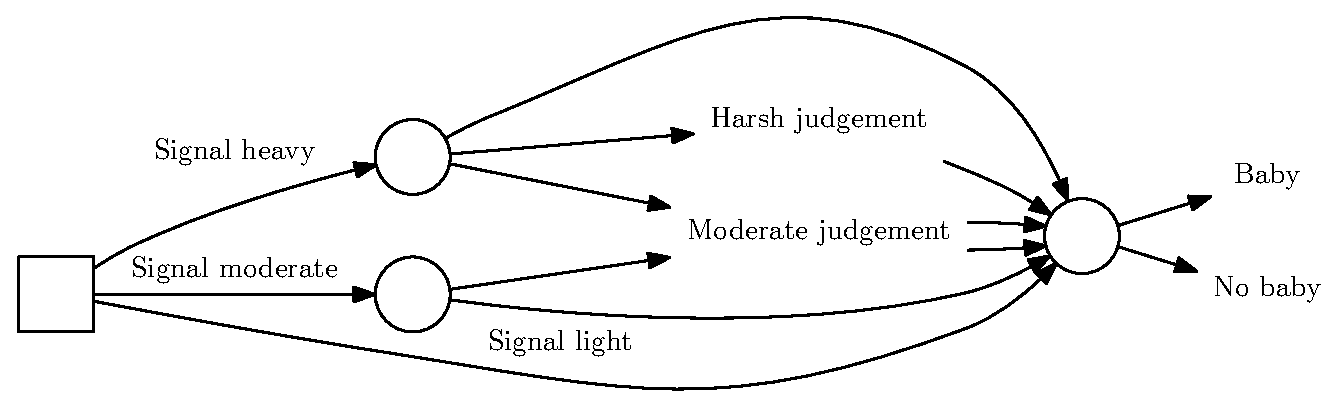
\includegraphics[width=119mm]{figures/women_influence}}
\vskip\baselineskip
\subfloat[Midwives]{\includegraphics[width=119mm]{figures/mw_influence}}
\caption{Influence diagrams, showing the game broken into two decision problems. Squares indicate a decision node, while circles are (from the perspective of the agent) chance nodes}

\label{fig:decision_problems}
\end{figure}


The precise structure of the decision problem is to some extent dependent on the decision rule in use, for example the Lexicographic heuristic rule is concerned only with a direct relationship between action and consequence. However, the literal translation from game to decision problem for women yields two chance nodes. As a result, solving this using the heuristic approach requires that the nodes be combined. By the same token, an arbitrarily complex problem could be resolved by rules without this limitation. This is significant, in that the decision problem is an individual agent's model of the situation, which might not be expected to correspond perfectly with the true situation.

From this position, simulating play, and augmenting the basic conjecture is easily achievable, since together the game, and the decision rules specify the basis for a simulation model. In the disclosure game case, we make additional stipulations on how many games agents play, order of play, the circumstances under which agents observe true types, and the structure of agent populations amongst others. 

\begin{comment}
At the end of a game, each player receives a payoff dependent on the actions and types of both players. Because both women and midwives have an interest in the outcome of the pregnancy, and would prefer a healthy baby, the payoff has a common interest component. Hence, both players receive a payoff based on the outcome of pregnancy, but women bear a social cost dependent on the signal they sent and the midwife's reaction to it. Similarly, midwives pay a cost if they refer to a specialist, mirroring the organisational cost of non-routine care. Table \ref{tab:Payoff-matrix} shows the three payoff matrices which together describe the game.



Taken together, this leads to a game tree that is relatively complex (figure \ref{fig:simple_tree} shows a simplified representation, with a detailed view of one branch in figure \ref{fig:zoom_tree}) even at the subgame level. 

As an example, consider the challenge faced by an agent of the heavy drinking type. In order to get the best health outcome, they must be referred and would ideally achieve this without paying any social cost at all. The best move depends on the type, and beliefs of the midwife. For example, a particularly unlucky scenario might be for the midwife to not only be of a harshly judgemental disposition, but to believe that no women really need to be referred. Even a relatively weak belief in this possibility can make the honest signal look like an unwarranted risk.

Rather than attempt to solve for equilibria, agents treat this two player game as taking place against nature, along the lines of adversarial risk analysis \citep{RiosInsua2009}. This effectively translates the game to a pair of decision problems (figure \ref{fig:decision_problems}), which agents attempt to resolve at each turn using a simple decision rule, given their prior beliefs and experience of play.

\begin{figure}[H]
\begin{adjustbox}{center}
\includegraphics[width=119mm]{figures/rounded_clover_infosets}
\end{adjustbox}
\caption{Simplified game tree. Arrows correspond to two moves by nature, followed by women, and midwives respectively. Line weight distinguishes between information sets, and possible moves, corresponding to ascending player types. For midwives, referral is shown by a heavier arrow. Light terminal nodes indicate that the game may repeat from that point, and black nodes are exits}

\label{fig:simple_tree}
\end{figure}

\begin{figure}[H]
\begin{adjustbox}{center}
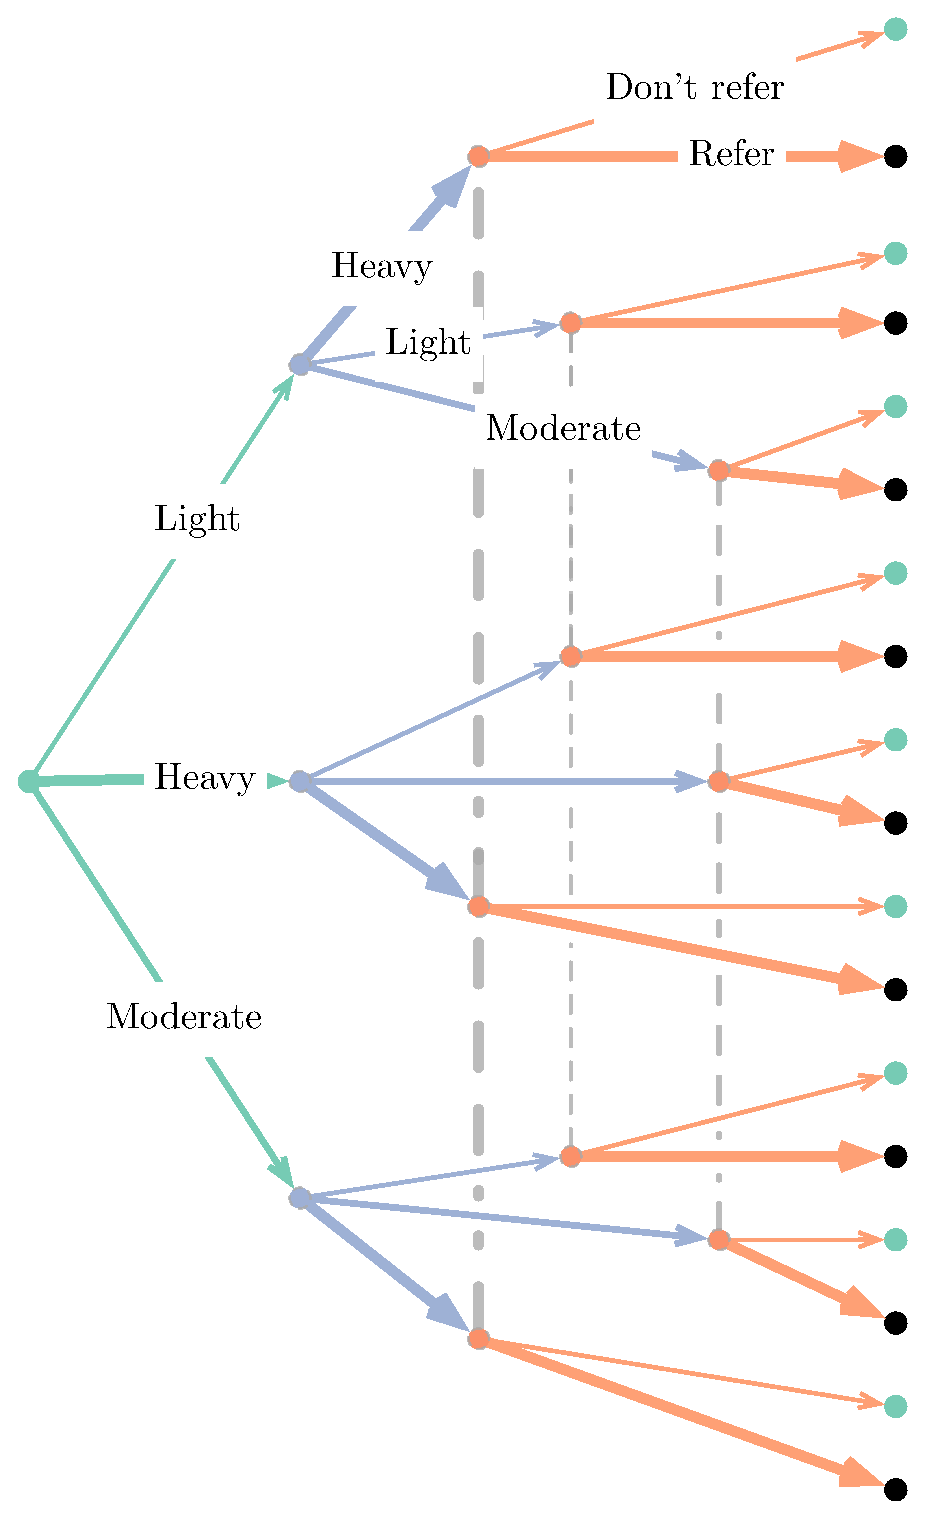
\includegraphics[width=119mm]{figures/tree_zoom}
\end{adjustbox}
\caption{Detail view of a single game tree branch, showing the possible moves by each player, with information sets for midwives}

\label{fig:zoom_tree}
\end{figure}

%Might belong in a more methody bit? Read some stuff to check..
To formally define the game, let \(N = \{m, w\}\) be the set of players each with a private type \(\theta_{i} \in \Theta\), and a set of types \(\Theta=\{l, m, h\}\), with pure strategies \(A_{m}=\{r,n\}, A_{w}=\{l, m, h\}\). Here, \(\{l, m, h\}\) correspond to light, moderate, and heavy alcohol consumption for women, and non-judgemental, moderately judgemental, and harshly judgemental for midwives. Midwives' pure strategies \(\{r,n\}\) are to refer, or do nothing, and those for women are to signal that they have one of the possible drinking patterns.
Additionally define two utility functions - 
\begin{equation}
u_{w}(s_{w}, s_{m}, \theta_{w}, \theta_{m})=X_{s, s_{w}, \theta_{m}} + X_{h, \theta_{w}, s_{m}}
\end{equation} 
\begin{equation}
u_{m}(s_{w}, s_{m}, \theta_{w})=X_{h, \theta_{w}, s_{m}} + X_{c, \theta_{w}, s_{m}},
\end{equation} with $X_{c}$, $X_{h}$, and $X_{s}$ being the payoff matrices as in table \ref{tab:Payoff-matrix}, $s_{w}$ and $s_{m}$ denoting a specific signal by a woman, and referral response by a midwife. Lastly let \(p_{w}(l, m, h)\), \(p_{m}(l, m, h)\) be distributions over types of women, and midwives respectively.


As noted, rather than solve the game, we allow populations of agents to play it, and hence stipulate further that women are drawn in order from a queue of \(n_{w}\) women (where \(n_{w}=1000\) in all simulations), and play against a midwife chosen at random from a population of \(n_{m}\) (\(n_{m}=100\)). They play for a maximum of \(r_{w}\) rounds (\(r_{w}=12\) following the routine number of ante-natal appointments in the UK \citep{NICE2010a}) or until they are referred, and a new player is drawn from the same distribution that produced the original players to replace them. If they are not referred, they rejoin the back of the queue after their appointment. In either case, they are informed of their payoff after each round and update their beliefs accordingly using one of the rules described in section \ref{sub:the_agents}.

Midwives play for \(r_{m}\) rounds (\(r_{m}=1000\) in all experiments), and conduct appointments in parallel, i.e. if there are 5 midwives, then five women are drawn from the queue and assigned at random to the midwives. 
Unlike women, midwives are only informed of their payoff if they choose to make a referral. Both groups of agents have perfect recall, and midwives are assumed to retrospectively update their observations if they make a referral after a number of appointments.
\end{comment}
%!TEX root = disclosure_game.tex

\section{Simulation Schedule}
\label{app:sim_schedule}

In this section we give the step by step process for a single run of the disclosure game simulation.

\begin{enumerate}
\item Generate 1000 women, and place them in a queue
\item Generate 100 midwives.
\item For each round of the game
\begin{enumerate}
	\item Take 100 women from the queue
	\item Pair each one with a random midwife
	\item For each pair
	\begin{enumerate}
		\item Woman sends a signal
		\item Midwife refers or not based on the signal
		\item Woman is informed of their payoff, the midwife's type, and whether they are referred
		\item The woman updates her beliefs
		\item The midwife stores the game in their memory
		\item If the woman is referred
		\begin{enumerate}
			\item The midwife is informed of the woman's true type
			\item The midwife retrospectively updates their beliefs using the true type, and memories of any games with this woman
			\item The midwife is now eligible to share their memories of games with this woman
		\end{enumerate}
	\end{enumerate}
	\item Women who have not been referred, or had their baby join the back of the queue
	\item Generate new women to replace those referred, or delivered
	\item Add new women to the back of the queue
	\item For each referred or birthed woman
	\begin{enumerate}
		\item With probability p, their memory of games is shared with the active women
		\item They are removed from simulation
	\end{enumerate}
	\item The active women update their beliefs
	\item For each midwife with information to share
	\begin{enumerate}
		\item With probability p, their memory of games with the referred woman is shared
		\item The memory is no longer eligible to be shared
	\item The midwives update their beliefs
	\end{enumerate}
\end{enumerate}
\end{enumerate}
\section{Agent Examples}
\label{sec:agent_eg}

This section provides a worked example for the learning and decision process of each agent model, focusing on the behaviour of the signalling agent.

\subsection{Lexicographic Heuristic}
\label{sub:lexico_eg}

As an example, take a light drinker who has played three rounds with a succession of particularly judgemental midwives, signalling honestly in two and claiming to be a moderate drinker in one. The most common outcome of the honest signal was a payoff of 10, which is clearly preferable to the 9 gained by claiming to be moderate. On that basis, they choose to signal honestly.

\subsection{Bayesian Payoff}
\label{sub:payoff_eg}

If we take our light drinker from the lexicographic case, and assume that they began with an uninformative prior. The 6 possible signal-payoffs pairings are then \([(l,10),(m,10),(h,10),(m,9),(h,9),(h,8)]\), with \(\alpha_{i}=1\) for all \(i\). After playing the three rounds, \(n_{l,10}=2\), and \(n_{m,9}=1\).

The agent then evaluates \(R_{w}\) for each signal, e.g. for the light signal:

\begin{equation*}
\begin{aligned}
X &= \{10\}\\
R_{w}(l) &= \sum_{x \in X} -xp(x | l) = -10p(10 | l)\\
R_{w}(l) &= -10(\frac{\alpha_{l,10}+n_{l,10}}{\sum_{j}(\alpha_{j}+n_{j})}) = -10(\frac{1+2}{1+2})\\
R_{w}(l) &= -10(\frac{3}{3}) = -10
\end{aligned}
\end{equation*}

and by the same method, \(R_{w}(m)=-9\frac{1}{3}\), and \(R_{w}(h)=-9\), concluding that signalling honestly is the best move.

\subsection{Bayesian Risk Minimisation}
\label{sub:bayes_eg}

Returning to our example agent, under this model the type of the midwife becomes salient, hence \(n_{h}=3\), and \(n_{l,n}=2\), \(n_{m,n}=1\). Their prior beliefs remain uninformative, i.e. \(\alpha_{j} = 1, j \in \{l,m,h\}\), \(\alpha_{i,j}=1,i \in \{r,n\}, j \in \{l,m,h\}\). As before, the agent evaluates \(R_{w}\) for the three signals, and the process for the light signal is given below -

\begin{equation*}
\begin{aligned}
R_{w}(l, l) &= \sum_{i\in A_{m}}\sum_{j\in \Theta} -u_{w}(l, i, l, j)p(j)p(i | l)\\
R_{w}(l, l) &= -u_{w}(l, r, l, l)p(l)p(r | l) - u_{w}(l, n, l, l)p(l)p(n | l) - u_{w}(l, r, l, m)p(m)p(r | l) - u_{w}(l, n, l, m)p(m)p(n | l) \\
&\phantom{{}=1}- u_{w}(l, r, l, h)p(h)p(r | l) - u_{w}(l, n, l, h)p(h)p(n | l)\\
u_{w}(l, i, l, j) &= 10\\
R_{w}(l, l) &= -10p(l)p(r | l) - 10p(l)p(n | l) - 10p(m)p(r | l) - 10p(m)p(n | l) - 10p(h)p(r | l) - 10p(h)p(n | l)\\
p(l) &= \frac{1 + 0}{1 + 1 + 1 + 3} = \frac{1}{6}\\
p(m) &= \frac{1 + 0}{1 + 1 + 1 + 3} = \frac{1}{6}\\
p(h) &= \frac{1 + 3}{1 + 1 + 1 + 3} = \frac{2}{3}\\
p(r | l) &= \frac{1 + 0}{1 + 1 + 2} = \frac{1}{4}\\
p(n | l) &= \frac{1 + 2}{1 + 1 + 2} = \frac{3}{4}\\
R_{w}(l, l) &= -10\cdot \frac{1}{6} \cdot \frac{1}{4} - 10\cdot \frac{1}{6} \cdot \frac{3}{4} - 10\cdot \frac{1}{6} \cdot \frac{1}{4} - 10\cdot \frac{1}{6} \cdot \frac{3}{4} - 10\cdot \frac{2}{3} \cdot \frac{1}{4} - 10\cdot \frac{2}{3} \cdot \frac{3}{4}\\
&= -10
\end{aligned}
\end{equation*}

and similarly for moderate (\(R_{w}(m,l)=-9\frac{1}{3}\)), and heavy (\(R_{w}(h,l)=-8\frac{1}{2}\)) signals, once again concluding that honesty is the better option.

\subsection{Descriptive Decision Theory}
\label{sub:cpt_eg}

Once again, we return to the light drinker example.  The inferential aspects are identical with the more complex Bayesian risk minimisation algorithm, hence \(p(j)p(i | l)\), and \(u_{w}(l, i, l, j)\) remain the same, but the agent additionally calculates $v(u_{w}(l, i, l, j))w^{+}(p(j))w^{+}(p(i | l))$. For the \ac{CPT} parameters, the values are those originally given by \citet{Tversky1992} and used in the actual simulations which are given fully in table \ref{tab:cpt_params}.

\begin{table}
\begin{tabular}{|l | l | c|}
\hline
Name & Description & Value \\ \hline
\(\gamma\) & Probability weighting for gains  & 0.61 \\ \hline
\(\delta\) & Probability weighting for losses &  0.69\\ \hline
\(\alpha\) & Power for gains  & 0.88 \\ \hline
\(\beta\) & Power for losses & 0.88 \\ \hline
\(\lambda\) & Loss aversion &  2.25 \\ \hline
\end{tabular}
\caption[Table caption text]{\ac{CPT} parameters. \label{tab:cpt_params}}
\end{table}

\begin{equation*}
\begin{aligned}
\alpha &= 0.88\\
\gamma &= 0.61\\
p(l) &= \frac{1}{6}\\
p(m) &= \frac{1}{6}\\
p(h) &= \frac{2}{3}\\
p(r | l) &= \frac{1}{4}\\
p(n | l) &= \frac{3}{4}\\
u_{w}(l, i, l, j) &= 10\\
f&=(10;\frac{1}{24},10;\frac{1}{8},10;\frac{1}{24},10;\frac{1}{8},10;\frac{1}{6},10;\frac{1}{2})\\
f^{+}&=f,f^{-}=()\\
n &= 5\\
v(u_{w}) &= f(u_{w}) = u_{w}^\alpha\\
v(u_{w}) &= 10^{0.88} = 7.59\\
\pi_{0}^{+}&=w^{+}(\frac{1}{24} + \frac{1}{8} + \frac{1}{24} + \frac{1}{8} + \frac{1}{6} + \frac{1}{2}) - w^{+}(\frac{1}{8} + \frac{1}{24} + \frac{1}{8} + \frac{1}{6} + \frac{1}{2})=w^{+}(1) - w^{+}(\frac{23}{24})\\
&=0.19\\
\pi_{1}^{+}&=w^{+}(\frac{1}{8} + \frac{1}{24} + \frac{1}{8} + \frac{1}{6} + \frac{1}{2}) - w^{+}(\frac{1}{24} + \frac{1}{8} + \frac{1}{6} + \frac{1}{2})=w^{+}(\frac{23}{24}) - w^{+}(\frac{5}{6})\\
&= 0.17\\
\pi_{2}^{+}&=w^{+}(\frac{1}{24} + \frac{1}{8} + \frac{1}{6} + \frac{1}{2}) - w^{+}(\frac{1}{8} + \frac{1}{6} + \frac{1}{2})=w^{+}(\frac{5}{6}) - w^{+}(\frac{19}{24})\\
&= 0.04\\
\pi_{3}^{+}&=w^{+}(\frac{1}{8} + \frac{1}{6} + \frac{1}{2}) - w^{+}(\frac{1}{6} + \frac{1}{2})=w^{+}(\frac{19}{24}) - w^{+}(\frac{2}{3})\\
&= 0.09\\
\pi_{4}^{+}&=w^{+}(\frac{1}{6} + \frac{1}{2}) - w^{+}(\frac{1}{2})=w^{+}(\frac{2}{3}) - w^{+}(\frac{1}{2})\\
&= 0.09\\
\pi_{5}^{+}&=w^{+}(\frac{1}{2})\\
&= 0.42\\
V(f) &= V(f^{+}) + V(f^{-}) = V(f^{+}) + 0\\
V(f^{+}) &= \sum_{i}^{n}\pi_{i}^{+}(f^{+})v_{i}^{+}(f^{+}) = 7.59
\end{aligned}
\end{equation*}


And as before, following the same process for moderate, and heavy signals which yields respectively 7.14, and 6.22, the agent chooses the higher valued action and sends an honest signal.
%!TEX root = disclosure_game.tex

\chapter{Supplementary Figures}
\label{app:additional_figures}

\begin{figure}[H]
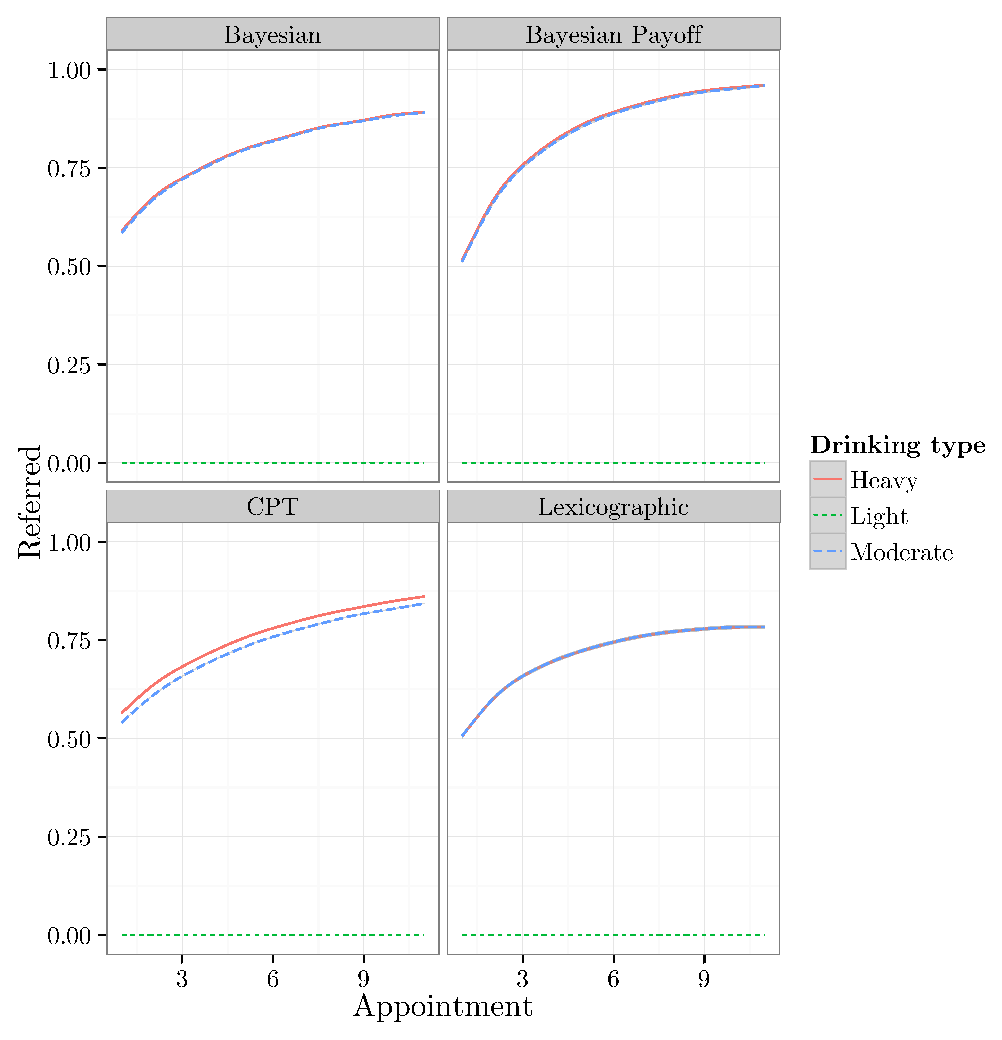
\includegraphics[width=100mm]{ref_plot}
\caption{Average fraction of population referred by each appointment, after 1000 rounds, mean with 95\% confidence limit over 1000 runs. Note that the large number of runs leads to very tight confidence intervals.\label{fig:ref_plot}}
\end{figure}
%!TEX root = disclosure_game.tex
%Include the descent into chaos bit
\section{Sensitivity Analysis}
\label{app:sensitivity_results}

\subsubsection{Median Moderate Drinker Signalling}

\begin{table}[h!]
\center
\begin{tabular} {|l | l | l | l | l | l |}
\hline
Parameter & Description & Lexicographic & Bayesian Payoff & Bayesian & \ac(CPT) \\ \hline
\(p_{w}(m)\) & Proportion of moderate drinkers & 0.367 & 1.145 \\ \hline
\(p_{w}(l)\) & Proportion of light drinkers & 10.080 & 37.750 \\ \hline
\(p_{m}(m)\) & Proportion of moderate midwives & 6.715 & 13.017\\ \hline
\(p_{m}(l)\) & Proportion of non-judgemental midwives & 43.942 & 1.655 \\ \hline
\(q_{w}\) & Probability of women sharing & 0.198 & 5.527 \\ \hline
\(w_{w}\) & Weight of shared information for women & 0.355 & 13.025 \\ \hline
\(q_{m}\) & Probability of midwives sharing & 0.145 & 0.667 \\ \hline
\(w_{m}\) & Weight of shared information for midwives & 0.118 & 0.376 \\ \hline
\(x_{h}\) & Health payoff for healthy delivery & 0.457 & 9.618 \\ \hline
\(s_{i}[a_{i}]:s_{i}[a_{\neg i}]\) & Psuedo-count favouring honesty & 0.140 & 7.537 \\ \hline
\end{tabular}
\caption[Table caption text]{Median moderate drinker signalling parameter sensitivity. \label{tab:sa_results_sig}}
\end{table}

\begin{table}[h!]
\center
\begin{tabular} {|l | l | l | l | l | l |}
\hline
Rule & \(\sigma^2\) & Nugget \(\sigma^2\) & Mean output & Total output variance & Code uncertainty & RMSSE \\ \hline
Lexicographic & 0.834 & 0.131 &  0.817 & 0.012 & 0.252 & 1.746 \\ \hline
Bayesian Payoff & 1.667 & 0.475 &  0.662 & 0.003 & 0.181 & 3.12 \\ \hline
Bayesian & 0.834 & 0.131 &  0.817 & 0.012 & 0.252 & 1.746 \\ \hline
\ac{CPT} & 0.834 & 0.131 &  0.817 & 0.012 & 0.252 & 1.746 \\ \hline
\end{tabular}
\caption[Table caption text]{Median moderate drinker signalling emulator statistics. \label{tab:sa_emulator_sig}}
\end{table}

\subsubsection{Median Between Groups IQR}

\begin{table}[h!]
\center
\begin{tabular} {|l | l | l | l | l | l |}
\hline
Parameter & Description & Lexicographic & Bayesian Payoff & Bayesian & \ac(CPT) \\ \hline
\(p_{w}(m)\) & Proportion of moderate drinkers & 0.367 & 1 \\ \hline
\(p_{w}(l)\) & Proportion of light drinkers & 10.080 & 1 \\ \hline
\(p_{m}(m)\) & Proportion of moderate midwives & 6.715 & 1 \\ \hline
\(p_{m}(l)\) & Proportion of non-judgemental midwives & 43.942 & 1 \\ \hline
\(q_{w}\) & Probability of women sharing & 0.198 & 1 \\ \hline
\(w_{w}\) & Weight of shared information for women & 0.355 & 1 \\ \hline
\(q_{m}\) & Probability of midwives sharing & 0.145 & 1 \\ \hline
\(w_{m}\) & Weight of shared information for midwives & 0.118 & 1 \\ \hline
\(x_{h}\) & Health payoff for healthy delivery & 0.457 & 100 \\ \hline
\(s_{i}[a_{i}]:s_{i}[a_{\neg i}]\) & Psuedo-count favouring honesty & 0.140 & 100:1 \\ \hline
\end{tabular}
\caption[Table caption text]{Median between groups IQR parameter sensitivity. \label{tab:sa_results_iqr}}
\end{table}

\begin{table}[h!]
\center
\begin{tabular} {|l | l | l | l | l | l |}
\hline
Rule & \(\sigma^2\) & Nugget \(\sigma^2\) & Mean output & Total output variance & Code uncertainty & RMSSE \\ \hline
Lexicographic & 0.834 & 0.131 &  0.817 & 0.012 & 0.252 & 1.746 \\ \hline
Bayesian Payoff & 0.834 & 0.131 &  0.817 & 0.012 & 0.252 & 1.746 \\ \hline
Bayesian & 0.834 & 0.131 &  0.817 & 0.012 & 0.252 & 1.746 \\ \hline
\ac{CPT} & 0.834 & 0.131 &  0.817 & 0.012 & 0.252 & 1.746 \\ \hline
\end{tabular}
\caption[Table caption text]{Median between groups IQR emulator statistics. \label{tab:sa_emulator_iqr}}
\end{table}

\subsubsection{Median Moderate Drinker Signalling IQR}

\begin{table}[h!]
\center
\begin{tabular} {|l | l | l | l | l | l |}
\hline
Parameter & Description & Lexicographic & Bayesian Payoff & Bayesian & \ac(CPT) \\ \hline
\(p_{w}(m)\) & Proportion of moderate drinkers & 0.367 & 1 \\ \hline
\(p_{w}(l)\) & Proportion of light drinkers & 10.080 & 1 \\ \hline
\(p_{m}(m)\) & Proportion of moderate midwives & 6.715 & 1 \\ \hline
\(p_{m}(l)\) & Proportion of non-judgemental midwives & 43.942 & 1 \\ \hline
\(q_{w}\) & Probability of women sharing & 0.198 & 1 \\ \hline
\(w_{w}\) & Weight of shared information for women & 0.355 & 1 \\ \hline
\(q_{m}\) & Probability of midwives sharing & 0.145 & 1 \\ \hline
\(w_{m}\) & Weight of shared information for midwives & 0.118 & 1 \\ \hline
\(x_{h}\) & Health payoff for healthy delivery & 0.457 & 100 \\ \hline
\(s_{i}[a_{i}]:s_{i}[a_{\neg i}]\) & Psuedo-count favouring honesty & 0.140 & 100:1 \\ \hline
\end{tabular}
\caption[Table caption text]{IQR of median moderate drinker signalling parameter sensitivity. \label{tab:sa_results_sig_iqr}}
\end{table}

\begin{table}[h!]
\center
\begin{tabular} {|l | l | l | l | l | l |}
\hline
Rule & \(\sigma^2\) & Nugget \(\sigma^2\) & Mean output & Total output variance & Code uncertainty & RMSSE \\ \hline
Lexicographic & 0.834 & 0.131 &  0.817 & 0.012 & 0.252 & 1.746 \\ \hline
Bayesian Payoff & 0.834 & 0.131 &  0.817 & 0.012 & 0.252 & 1.746 \\ \hline
Bayesian & 0.834 & 0.131 &  0.817 & 0.012 & 0.252 & 1.746 \\ \hline
\ac{CPT} & 0.834 & 0.131 &  0.817 & 0.012 & 0.252 & 1.746 \\ \hline
\end{tabular}
\caption[Table caption text]{IQR of median between groups IQR emulator statistics. \label{tab:sa_emulator_sig_iqr}}
\end{table}

\subsubsection{Between Groups IQR IQR}

\begin{table}[h!]
\center
\begin{tabular} {|l | l | l | l | l | l |}
\hline
Parameter & Description & Lexicographic & Bayesian Payoff & Bayesian & \ac(CPT) \\ \hline
\(p_{w}(m)\) & Proportion of moderate drinkers & 0.367 & 1 \\ \hline
\(p_{w}(l)\) & Proportion of light drinkers & 10.080 & 1 \\ \hline
\(p_{m}(m)\) & Proportion of moderate midwives & 6.715 & 1 \\ \hline
\(p_{m}(l)\) & Proportion of non-judgemental midwives & 43.942 & 1 \\ \hline
\(q_{w}\) & Probability of women sharing & 0.198 & 1 \\ \hline
\(w_{w}\) & Weight of shared information for women & 0.355 & 1 \\ \hline
\(q_{m}\) & Probability of midwives sharing & 0.145 & 1 \\ \hline
\(w_{m}\) & Weight of shared information for midwives & 0.118 & 1 \\ \hline
\(x_{h}\) & Health payoff for healthy delivery & 0.457 & 100 \\ \hline
\(s_{i}[a_{i}]:s_{i}[a_{\neg i}]\) & Psuedo-count favouring honesty & 0.140 & 100:1 \\ \hline
\end{tabular}
\caption[Table caption text]{IQR of median between groups IQR parameter sensitivity. \label{tab:sa_results_iqr_iqr}}
\end{table}

\begin{table}[h!]
\center
\begin{tabular} {|l | l | l | l | l | l |}
\hline
Rule & \(\sigma^2\) & Nugget \(\sigma^2\) & Mean output & Total output variance & Code uncertainty & RMSSE \\ \hline
Lexicographic & 0.834 & 0.131 &  0.817 & 0.012 & 0.252 & 1.746 \\ \hline
Bayesian Payoff & 0.834 & 0.131 &  0.817 & 0.012 & 0.252 & 1.746 \\ \hline
Bayesian & 0.834 & 0.131 &  0.817 & 0.012 & 0.252 & 1.746 \\ \hline
\ac{CPT} & 0.834 & 0.131 &  0.817 & 0.012 & 0.252 & 1.746 \\ \hline
\end{tabular}
\caption[Table caption text]{IQR of median between groups IQR emulator statistics. \label{tab:sa_emulator_iqr_iqr}}
\end{table}
\end{document}